
\documentclass[10pt, conference, compsocconf]{IEEEtran}  
                                                         


\IEEEoverridecommandlockouts                             
                                                         
                                                         
\overrideIEEEmargins

\usepackage[latin1]{inputenc}
\usepackage{makecell}
\usepackage{graphicx}
\usepackage{blindtext, graphicx}
\usepackage{multirow}
%\usepackage{algorithm}
\usepackage{algpseudocode}
\algdef{SE}[DOWHILE]{Do}{doWhile}{\algorithmicdo}[1]{\algorithmicwhile\ #1}%
\setcounter{secnumdepth}{4}
\usepackage[linesnumbered,ruled,vlined]{algorithm2e} 
\usepackage[first=0,last=9]{lcg}
\usepackage{color, colortbl}
\definecolor{Gray}{gray}{0.9}
\usepackage{tabularx} % in the preamble
\usepackage{tabu}
\usepackage{booktabs}
\usepackage[tight,footnotesize]{subfigure}
\usepackage[usenames,table]{xcolor}

\newcolumntype{P}[1]{>{\centering\arraybackslash}p{#1}}
\newcolumntype{M}[1]{>{\centering\arraybackslash}m{#1}}
\newcommand{\head}[1]{\textnormal{\textbf{#1}}}


\title{\LARGE \bf
Host Hypervisor Trace Mining for Virtual Machine Workload Characterization
}


\author{\IEEEauthorblockN{Hani Nemati\IEEEauthorrefmark{1}, Seyed Vahid Azhari\IEEEauthorrefmark{2}, and Michel R. Dagenais\IEEEauthorrefmark{3}}
\IEEEauthorblockA{Department of Computer and Software Engineering,\\ Polytechnique Montreal, Quebec, Canada \\
Email: \{\IEEEauthorrefmark{1}hani.nemati@polymtl.ca,\IEEEauthorrefmark{2}azharivs@gmail.com,\IEEEauthorrefmark{3}michel.dagenais@polymtl.ca}}


\begin{document}



\maketitle
\thispagestyle{empty}
\pagestyle{empty}


%%%%%%%%%%%%%%%%%%%%%%%%%%%%%%%%%%%%%%%%%%%%%%%%%%%%%%%%%%%%%%%%%%%%%%%%%%%%%%%%
\begin{abstract}

The efficient operation and resource management of multi-tenant data centers hosting thousands of services is a demanding task that requires precise and detailed information regarding the behaviour of each and every virtual machine (VM). Often, coarse measures such as CPU, memory, disk and network usage by VMs are considered in grouping them onto the same physical server, as detailed measures would require access to the guest operating system (OS) which is not feasible in a multi-tenant setting.

In this paper, we propose host level hypervisor tracing as a non-intrusive means to extract useful features that can provide for fine grain characterization of VM behaviour. In particular, we extract VM blocking periods as well as virtual interrupt injection rates to detect multiple levels of resource intensiveness. In addition, we consider resource contention rate due to other VMs and the host, along with reasons for exit from non-root to root privileged mode revealing useful information about the nature of the underlying VM workload. We also use tracing to get information about rate of process and thread preemption in each VM extracting process and thread contention as another feature set. We then employ various feature selection strategies and assess the quality of the resulting workload clustering. Notably, we adopt a two stage feature selection approach in addition to a one shot clustering scheme. Moreover, we consider inter-cluster and intra-cluster similarity metrics such as silhouette score to discover distinct groups of workloads as well as workload groups with significant overlap. This information can be used by 1) data center administrators to gain deep visibility into the nature of various VMs running on their infrastructure, 2) performance engineers to assist root cause analysis of VM issues and 3) IaaS provider to help in resource management based on VM behavior. 


\end{abstract}


\begin{IEEEkeywords}
VM Clustering, Workload characterization, performance analysis, tracing, vCPU states, K-Means, Machine Learning.
\end{IEEEkeywords}

%%%%%%%%%%%%%%%%%%%%%%%%%%%%%%%%%%%%%%%%%%%%%%%%%%%%%%%%%%%%%%%%%%%%%%%%%%%%%%%%
\section{Introduction}

Introduction goes here. 

%%%%%%%%%%%%%%%%%%%%%%%%%%%%%%%%%%%%%%%%%%%%%%%%%%%%%%%%%%%%%%%%%%%%%%%%%%%%%%%%
\section{Related Work}



%%%%%%%%%%%%%%%%%%%%%%%%%%%%%%%%%%%%%%%%%%%%%%%%%%%%%%%%%%%%%%%%%%%%%%%%%%%%%%%%


\section{VM Features and Types Selection}

\subsection{VMX Operation}

Intel processors (like AMD processors) provide support for virtualization by Virtual Machine eXtensions (VMX) instructions set (AMD
supports Secure Virtual Machine (SVM) instructions set). There are two types of VMX operation: \textbf{VMX root} operation and \textbf{VMX non-root} operation.  Privileged instruction executed by VM causes a VM exit to VMX root mode to pass the control to Virtual Machine Monitor (VMM) in order to execute the instruction in a safe environment.  After handling the privileged instruction, the VM resumes to VMX non-root. The transition between VMX root to VMX non-root is called VM entry and the transition between VMX non-root to VMX root is called VM exit.  The VMM keeps track of transitions by updating an in-memory data structure called Virtual-Machine Control Structure (VMCS). VMM creats different VMCS for each vCPU and uses \texttt{VMREAD}, \texttt{VMWRITE} and \texttt{VMCLEAR} instructions to update VM information. Each VM exit comes with the exit number which showing the reason of exit. The number could be used to reveal information about running application inside VM. 

\subsection{Virtual Interrupt Injection}

Virtual Machine Extensions (VMX), instructions on processors with x86 virtualization, supports virtual interrupt (\texttt{virq}) injection into VM by filling VM-entry interrupt-information field in Virtual Machine Control Structure (VMCS). Interrupt injection includes software interrupt, internal interrupt, and external interrupt. Then, the processor uses interrupt information field to deliver virtual interrupt through the VM Interrupt Descriptor Table (IDT).  Usually, the virq will be injected to guest during next VM exit by emulating the \texttt{LAPIC} register. Once the VM resumed, the pending interrupt is executed by looking up the VM's \texttt{IDT}. After handling the interrupt, during the next VM exit, the processor performs End Of Interrupt \texttt{EOI} virulization to update guest interrupt status. Looking at injected interrupt reveals useful information about running application inside the VM. We elaborate more on the extracted metrics from injected \texttt{virq} in the next subsection. 



\begin{figure}[h]
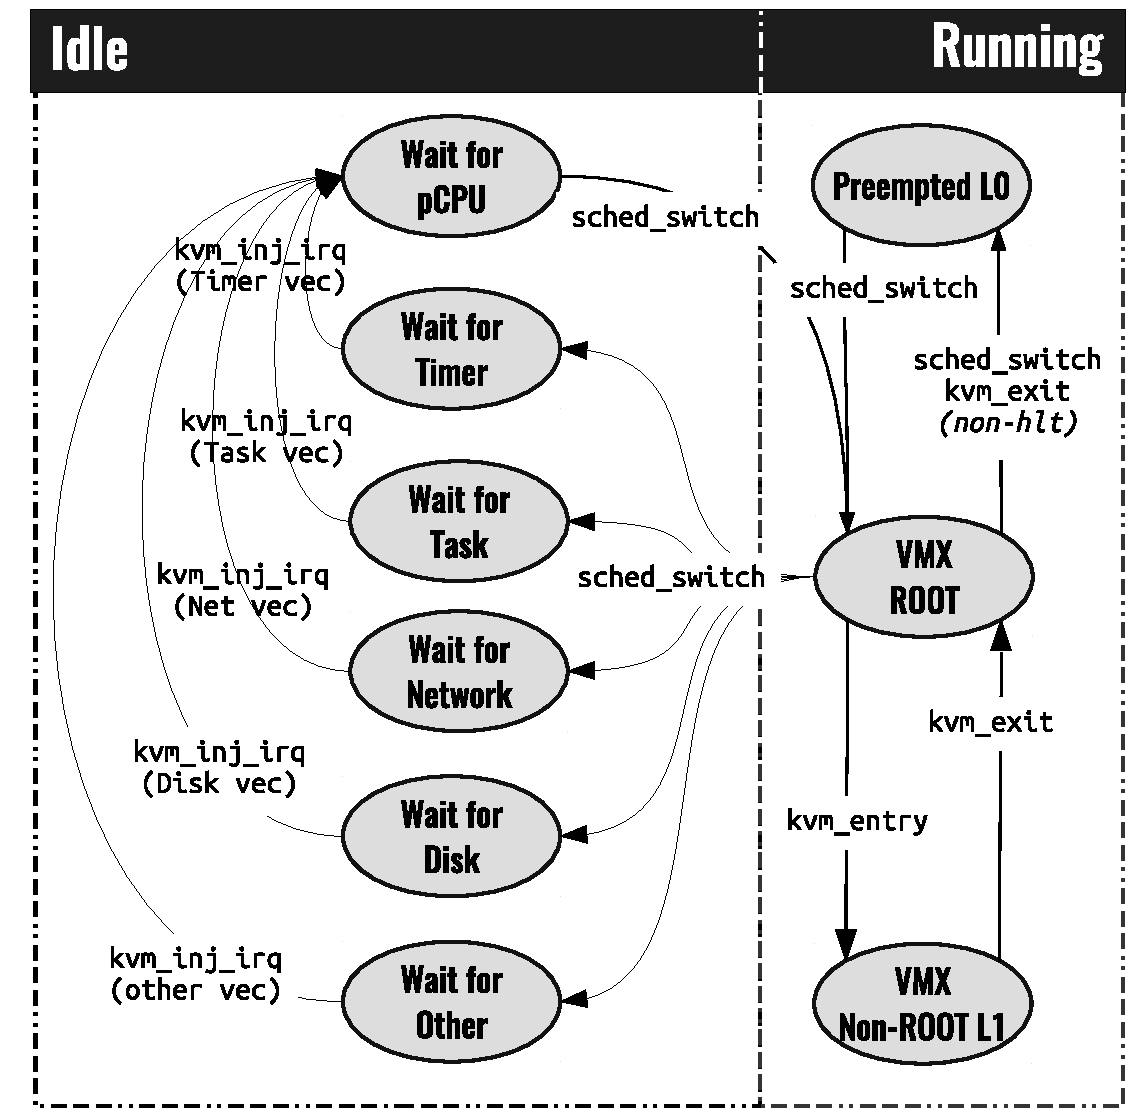
\includegraphics[width=0.45\textwidth]{figs/states.pdf}
\caption{Virtual Machine virtual CPU State Transition}
\label{fig:state}
\end{figure}

\subsection{VM Machine States Analysis}

Figure \ref{fig:state} shows different possible states of virtual CPU of a VM and their condition to reach them. Like physical CPU (pCPU) each vCPU could be either in running state or idle state. As we mentioned before, while running a privileged instruction the VM exit to VMX root mode to execute the instruction and then with vm entry it resumes the VM. In addition, from VM point of view, VM assumes that it is the only one using the whole resources. In fact, VM shares its resources and that causes resource contention. The preemption state is when the host scheduler decides to take pCPU and gives it to another VM or process. It halts executing VM for a while without notifying the VM. Consequently, the VM process is in running state inside VM but it does not execute any instruction. The preemption state is one of the state that could not be shown from inside VM. Other than running states, analyzing idle states bring useful information. When a vCPU is being scheduled out voluntary, it execute \texttt{hlt} instruction which is a privileged instruction. This instruction causes an exit to VMX root and the host scheduler realize that the vCPU thread should be schedule out of pCPU. In this state the vCPU
waits for a signal to be waken up. The host scheduler wakes up the vCPU thread mainly for following reasons. \textbf{First}, a process inside the VM sets a timer and the timer is fired (Timer Interrupt). \textbf{Second}, inter process communication wakes up a process (IPI interrupt). \textbf{Third}, a process inside VM waits for incoming packet from remote process (Network Interrupt). \textbf{Fourth}, a process inside the VM waits for Disk (Disk interrupts). Other than Timer, IPI, Network, and Disk interrupts, the VM could wait for another device (with different virq number) which could be labeled as wait for other. The wait for X states along with running state will be used by our feature extraction mechanism to collect information about running VM. 

In order to detect the reason of waking up, we introduce Wake-up Reason Analysis (WRA). The pseudocode for the WRA algorithm is depicted in Algorithm \ref{alg:wra}. The WRA algorithm receives a sequence of events as input and detects the reason of wait for a vCPU of given VM. Whenever a VM has something to execute, it asks for pCPU from host scheduler. Receiving \texttt{sched\_wakeup} event shows that the VM ask for a pCPU and the state of vCPU is updated to waiting for pCPU. Event \texttt{sched\_in} shows a vCPU is scheduled in on pCPU, but still it is in waiting state to run. We name this state wait for vCPU. Before running the vCPU on pCPU the hypervisor injects interrupt into the VM. These interrups are the key of our analysis. The event related to interrupt injection is \texttt{vm\_inj\_virq}. The vec field in this event is compared with the Task, Timer, Disk, and Network interrupt number. The reason of waiting is updated based on the \textit{vec} number. The different interrupt numbers are being retrieved by following the pattern of using device. This pattern is different between hypervisors.  

The \texttt{vcpu\_enter\_guest} event changes the vCPU state to running (Line \ref{wra:line:vcpu_running}). We also store the CR3 value in the payload of this event.  CR3 points to the page directory of a process in any level of virtualization, and could be used as an unique identifier of a process. As we mentioned before, a running vCPU could be preempted either in host level (L0) or guest level (L1). If the last exit is \texttt{hlt}, which means that the VM runs the idle thread, the state will be modified as wait for reason. In the other case of exit number, the state will be changed to preempted (Line \ref{wra:line:sched_switch:preemptedL0}). The preemption L1 happens when the process inside the VM is preempted by guest scheduler. In this case the cr3 will be changed with out running \texttt{hlt} instruction (Line \ref{wra:line:process:preemptedL1}).  

\begin{algorithm} 
  \uIf{event == $sched\_in$}{
	$vCPU_j^{State}$ = vCPU-root\;\label{wra:line:vcpu_wakeup}
	last\_exit = getLastExit($vCPU_j$) \;
	\uIf{last\_exit != hlt} {
  	    $vCPU_k^{State}$ = Preempted\_L0 \label{wra:line:sched_switch:preemptedL0}
  	} \uElse {
  	    $vCPU_k^{State}$ = waiting\_for\_reason \label{wra:line:sched_switch:waiting}
  	}
  }
   \uElseIf{ event == $vm\_exit$}{
   putLastExit($exit\_number$)\;
  	$vCPU_j^{State}$ = vCPU-root \;\label{wra:line:vcpu_root}
  }
  \uElseIf{ event == $sched\_wakeup$}{
  	$vCPU_j^{State}$ = pCPU-waiting \;\label{wra:line:pcpu_wakeup}
  }
  \uElseIf{ event == $vcpu\_enter\_guest$}{
    lastCR3 = getLastCR3($vCPU_j$)\;
    \uIf{lastCR3 != cr3} {
  	    $vCPU_j^{internal}$ = Preempted\_L1 \label{wra:line:process:preemptedL1}
  	} 
    $vCPU_j^{State}$ = vCPU-root\;\label{wra:line:vcpu_wakeup}
  	
    $vCPU_j^{State}$ = vCPU-non-root \;\label{wra:line:vcpu_running}
  	putLastCR3(c$r3$) \;\label{wra:line:cr3Store}
  }
  \uElseIf{ event == $sched\_out$}{
  	$vCPU_j^{State}$ = idle \;\label{wra:line:idle}
  }
 \uElseIf{ event == $vm\_inj\_virq$}{
 	\uIf{vec == Task Interrupt} {
 		Update State for $vCPU_j^{State}$ to Task\;\label{wra:line:task}
 	} 
 	\uElseIf{vec == Timer Interrupt} {
 	Update State for $vCPU_j^{State}$ to Timer\;\label{wra:line:Timer}
 	}
 	\uElseIf{vec == Disk Interrupt} {
 	Update State for $vCPU_j^{State}$ to Disk\;\label{wra:line:Disk}
 	}
 	\uElseIf{vec == Network Interrupt} {
 	Update State for $vCPU_j^{State}$ to Network\;\label{wra:line:Network}
 	}
 	\uElse{
 	Update State for $vCPU_j^{State}$ to Other
 	}
 }
\caption{Wakeup Reason Analysis Algorithm (WRA)}
\label{alg:wra}
\end{algorithm}

\subsection{Extracted Features}








\begin{table}
\caption{Notations}
\centering
\begin{tabular}{ll}
  \hline
  \rowcolor{Gray}
  \footnotesize \textbf{Term} & \footnotesize \textbf{Features collected by tracing} \\
  \hline
  \hline
  \footnotesize \textit{$W_{Disk}$} & \footnotesize Wait for Disk average time\\
  \footnotesize \textit{$W_{Net}$} & \footnotesize Wait for Net average time\\
  \footnotesize \textit{$W_{Timer}$} & \footnotesize Wait for Timer average time\\
  \footnotesize \textit{$W_{Task}$} & \footnotesize Wait for Task average time\\
  \footnotesize \textit{$E_{Root}$} & \footnotesize Root mode average time\\
  \footnotesize \textit{$E_{non-Root}$} & \footnotesize non-Root mode average time\\
  \footnotesize \textit{$FP_{VMVM}$} & \footnotesize The frequency of two VMs preempt each other\\
  \footnotesize \textit{$FP_{HostVM}$} & \footnotesize The frequency of host preempts a VM\\
  \footnotesize \textit{$FP_{VMProc}$} & \footnotesize The frequency of VM processes preempt each other\\
  \footnotesize \textit{$FP_{VMThread}$} & \footnotesize The frequency of VM threads preempt each other\\
  \footnotesize \textit{$f_{Disk}$} & \footnotesize The frequency of wait for Disk\\
  \footnotesize \textit{$f_{Net}$} & \footnotesize The frequency of wait for Net\\
  \footnotesize \textit{$f_{Timer}$} & \footnotesize The frequency of wait for Timer\\
  \footnotesize \textit{$f_{Task}$} & \footnotesize The frequency of wait for Task\\
  \footnotesize \textit{$N_{Exit}$} & \footnotesize The frequency of different VM exit reason\\
  \footnotesize \textit{$f_{Read}$} & \footnotesize The frequency of read from Disk\\
  \footnotesize \textit{$f_{Write}$} & \footnotesize The frequency of write to Disk\\
  \footnotesize \textit{$B_{Read}$} & \footnotesize Total Block Disk Read\\
  \footnotesize \textit{$L_{Read}$} & \footnotesize Total Latency Disk Read\\
  \footnotesize \textit{$B_{Write}$} & \footnotesize Total Block Disk Write\\
  \footnotesize \textit{$L_{Write}$} & \footnotesize Total Latency Disk Write\\
  \hline
\end{tabular}
\label{tab:notation}
\end{table}



\begin{table}
\caption{Needed Tracepoints for feature extraction}
\centering
\begin{tabular}{p{2.5cm}p{5.8cm}}
  \hline
  \rowcolor{Gray}
  \footnotesize \textbf{Tracepoint} & \footnotesize \textbf{Description} \\
  \hline
  \hline
  
  \footnotesize \texttt{sched\_wakeup}  & \footnotesize Wakeup and resume a task \\
  \footnotesize \texttt{vcpu\_enter\_guest}  & \footnotesize vCPU enters guest mode \\
  \footnotesize \texttt{vm\_exit}  & \footnotesize vCPU exits guest mode \\
  \footnotesize \texttt{vm\_inj\_virq}  & \footnotesize Inject virtual interrupt into VM \\
  \footnotesize \texttt{sched\_switch}  & \footnotesize  Scheduling out or in a process\\
    \hline
\end{tabular}
\label{tab:agent-base-tracepoints}
\end{table}

%%%%%%%%%%%%%%%%%%%%%%%%%%%%%%%%%%%%%%%%%%%%%%%%%%%%%%%%%%%%%%%%%%%%%%%%%%%%%%%%
\section{VM Workload Clustering Model}

%What is clustering, how it is unsupervised and that is an advantage and how it can group workloads and what is the benefit of that. What is Kmeans and how it is useful for euclidean globular shapes which is suitable for our extracted features. Centroids or prototypes and that we use them to represent our workload behaviour to the cloud admin.  put a few refs to Kmeans
We apply the Kmeans clustering algorithm \cite{kmeans1} to our set of sample vectors derived via the feature extraction process. Note that this is an unsupervised process as compared with classification and requires no training data set. A clustering approach groups VM workloads based on the actual workload distribution in the data center. Consequently, it potentially ``discovers'' interesting groups of VMs, as opposed to assigning a predefined label to them. Each sample $i$ represents some VM workload denoted by $VM_i$ as a vector of features, i.e.,  
%
\begin{equation}
VM_i = (f_{i1},f_{i2},...,f_{ij},...,f_{iM})
\label{eq:sample-vector}
\end{equation}

%Explain normalization performed over various features and why we need this
To allow for meaningful comparison, sample vectors are individually normalized using the $L2$ norm such that they become of equal magnitude \cite{Kmeans2}, that is,
%
\begin{equation}
\sum_{m=1}^{M} f_{im}^2 = 1,~\forall i=1..N.
\label{eq:l2-norm} 
\end{equation}

The Kmeans clustering algorithm will discover clusters $C_1,...,C_K$ of similar VMs over a sample matrix, $VM_{N,M}$, which includes one sample vector per row. In order to do this, we use the Euclidean distance metric over feature vectors to measure similarity among VM samples. Two VMs are grouped into the same cluster if their Euclidean distance is small. More formally, the Kmeans approach to clustering is based on the notion of centroids (a.k.a. prototypes), which are hypothetical sample points placed at the center of each cluster. Given a certain number of centroids, $K$, Kmeans will determine cluster membership for all samples such that the sum of squared distance from each sample $VM_i$ to its closest centroid $C_j$ is minimized over all set of samples \cite{kmeans3}. That is,
%
\begin{equation}
min \sum_{i=1}^{N} \sum_{k=1}^{M} (f_{ik} - c_{jk})^2 \label{eq:kmeans-obj}
\label{eq:kmeans-obj}
\end{equation}
%
where the solution to (\ref{eq:kmeans-obj}) will be $C_j = (c_{j1},...,c_{jk},...,c_{jM}), j=1..K$, which are the hypothetical coordinates of the $j^{th}$ centroid that is the closest to $VM_i$.

A distinct advantage of Kmeans is that each centroid (a.k.a. prototype) can be used to represent the workload of its cluster as discussed in Section \ref{sec:exp}. This provides condensed useful information of the bahavior of many VMs. 

%Explain how we evaluate a cluster and introduce silhouette score of samples, total and each cluster. Provide the relationship. What can be expected and what cannot be expected from it. What does it mean to have overlap, etc.
Furthermore, we need a measure to assess the suitability of a given clustering. There are an array of such measures introduced in the literature \cite{kmeans4}, which essentially characterize a clustering through its cohesion and/or separation. A cohesive clustering is one in which individual clusters consist of tightly packed very similar samples. Separation, on the other hand, evaluates how distinct clusters are well apart. Consequently, we adopt the ``silhouette'' score \cite{sil} which considers both cohesion and separation and is computed for a given sample $VM_i$ as,
%
\begin{equation}
s_i = \frac{out_i - in_i}{max(in_i,out_i)}
\label{eq:sil}
\end{equation}
%
Here, $in_i$ is the average distance of $VM_i$ to all other VM samples in its cluster, while $out_i$ is the minimum average distance between $VM_i$ and all other samples in clusters not containing $VM_i$. The value of silhouette coefficient lies between -1 and 1, where a positive large value is more desirable. We would like to have $in_i$ as close as possible to zero for a very cohesive cluster, and to have $out_i$ as large as possible representing very large separation from the closest neighbor cluster. A negative value $(in_i > out_i)$ is undesirable because it corresponds to when average distance to in-cluster samples exceeds minimum average distance to out-cluster samples. It should be noted that, while the quality of a clustering algorithm plays an important role in finding good clusters, having cohesive and well separated clusters also largely depends on the nature of the data and the distance metric. The silhouette coefficient can be averaged over a cluster or the entire samples to yield a silhouette score per cluster or for the entire clustering, respectively. 

%Our two stage approach where we first find very coarse clusters and then do further clustering on each.
We employ a two stage clustering approach, where the entire set of VMs are first grouped into a small number of clusters. We then apply a second stage clustering to each cluster discovered in the first stage to yield our final VM groups. Hence, each VM would be characterized by two numbers $(Ci,Cj)$ standing for the cluster it belongs to in the first and second stage, respectively. We believe this two stage approach provides better grouping of VM workloads by first performing a coarse grain characterization of VMs followed by more detailed clustering. It should be noted that, our clustering selection criteria is always guided by total silhouette score. That is, at any stage we select the clustering with maximum total silhouette score as the desired solution. 

%%%%%%%%%%%%%%%%%%%%%%%%%%%%%%%%%%%%%%%%%%%%%%%%%%%%%%%%%%%%%%%%%%%%%%%%%%%%%%%%
\section{Experimental Evaluation}\label{sec:exp}

\begin{table}
\caption{List of applications for workload generation}
\centering
\begin{tabular}{M{0.14\linewidth}M{0.30\linewidth}M{0.45\linewidth}}
  \hline
  \rowcolor{Gray}
  \footnotesize \textbf{Application Behavior} & \footnotesize \textbf{Application Name} & \footnotesize \textbf{Application Description} \\
  \hline
  \hline
    \footnotesize \rotatebox[origin=c]{90}{CPU} & \footnotesize Sysbench, Stress, Burn, Chess, Compress, encode, interBench, openSSL, smallpt, infinitLoop  & Bunch of well-konwn benchmarking tools for Linux to stress CPU including computing prime number, compressing files, video and audio encoding, mathematic operations \\  \hline
  \footnotesize  \rotatebox[origin=c]{90}{Disk} & \footnotesize Sysbench, Compress, dbench, dd, interBench, hdparam, fsMarker, aio, ioZone, pgbench-disk, pqlight, stream, tioBench & Include different testing toolkits for Disk I/O. These toolkits provide realistic scenario for reading/writing with different options to evaluate Disk I/O.  \\  \hline
   \footnotesize  \rotatebox[origin=c]{90}{Net} & \footnotesize  Wget, iperf, netperf, netping, netSpeedTest, scp, ab, httperf & Include real network applications in Linux. It covers web server, file transfer server, downloading file.    \\
  \hline
\end{tabular}
\label{tab:notation}
\end{table}

%%%%%%%%%%%%%%%%%%%%%%%%%
\begin{figure}[!htpb]
\centering
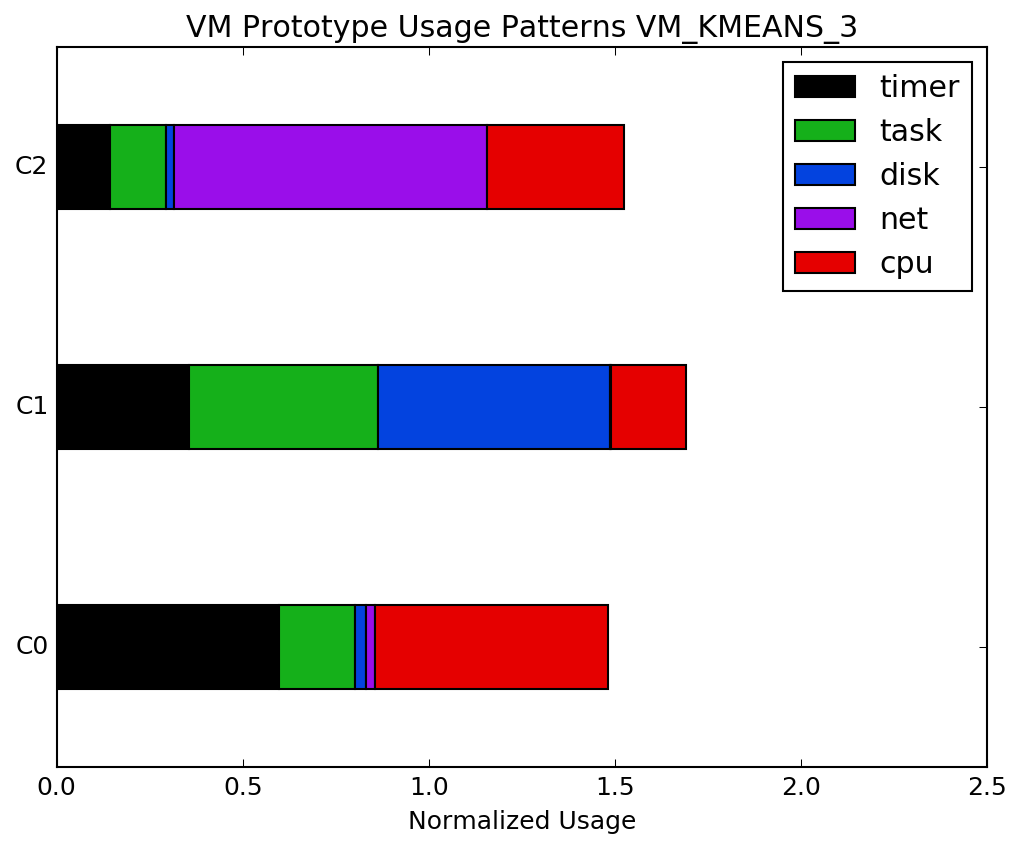
\includegraphics[width=0.45\textwidth]{figs/VM_KMEANS_3_centroids.png}
\caption{Characteristic of Workloads Discovered in First Stage of Clustering}
\label{fig:1st-centroids}
\end{figure}
%%%%%%%%%%%%%%%%%%%%%%%%%%%%
%Discuss the centroids found and say what each represents and why these are interesting. Also how we got to this three clusters by taking the one with the best silhouette score. 
In this section we presents results for the two stage clustering approach. For the results presented in this paper we have only used cpu usage and interrupt injection rate for network, disk, task, and timer interrupts as our feature vector. {\color{red} Hani: I think you missed the injection rates in your table}. At the first stage we found that applying Kmeans to find three coarse clusters would yield the best total silhouette score of 0.42 and per cluster silhouette of $C0=0.38, C1=0.35, C2=0.48$. Figure \ref{fig:1st-centroids} shows the three centroids obtained via the first stage clustering. Note that the feature vectors are normalized so that their absolute values are of no significance. 

Interestingly, three distinct groups of VMs are discovered in Figure \ref{fig:1st-centroids}. Cluster C0 is discovered to be CPU intensive as the prototype usage pattern includes large CPU and Timer interrupt injection rate. The large timer injection rate corresponds to many host scheduler preemptions which is characteristic of CPU intensive tasks that do not yield CPU. {\color{red} Hani: please check, elaborate and provide examples.} On the other hand, clusters C1 and C2 represent disk and network intensive VMs, respectively. An interesting observation is that unlike the network intensive VMs of C2, disk intensive VMs in C1 make significant use of task interrupt. This is an indication of disk VMs waiting more frequently for some task to finish I/O as opposed to network VMs which wait for some process on another machine. The information obtained via cluster prototypes can be used by cloud infrastructure administrator to guide resource management. {\color{red} Hani: please check, elaborate and provide examples.}

We next apply Kmeans to each of the first stage clusters independently and select the clustering with largest silhouette score. For our particular set of workload, this approach resulted in a total of 10 clusters. The first stage cluster C0 turns out to be best characterized as five distinct groups of VMs with a total silhouette score of 0.59. Figure \ref{fig:c0-sim} illustrates the similarity plot for the five clusters found in the second stage. Each point on both X and Y axis correspond to a particular VM which is labeled once on the Y axis. The label consists of a VM textual name followed by a slash and then the PID of the process running the VM. The second stage cluster index corresponding to this VM is enclosed in brackets at the end. 

Each point on the similarity plot presents the normalized euclidean distance defined as in (\ref{eq:similarity}) between VM feature vectors intersecting at that point. Note that $d_{ij}$ is the actual euclidean distance between VM $i$ and $j$, while $d_{max}$ and $d_{min}$ correspond to the maximum and minimum distances, respectively. It follows that the similarity score of any two VM is between zero and one. Interestingly, if VMs are sorted according to their cluster index, the similarity plot should resemble a block diagonal shape for cohesive and well separated clusters. 
%
\begin{equation}
sim_{ij} = 1-\frac{d_{ij}-d_{min}}{d_{max}-d_{min}}
\label{eq:similarity}
\end{equation}
%
%%%%%%%%%%%%%%%%%%%%%%%%%
\begin{figure*}[!htpb]
\centering
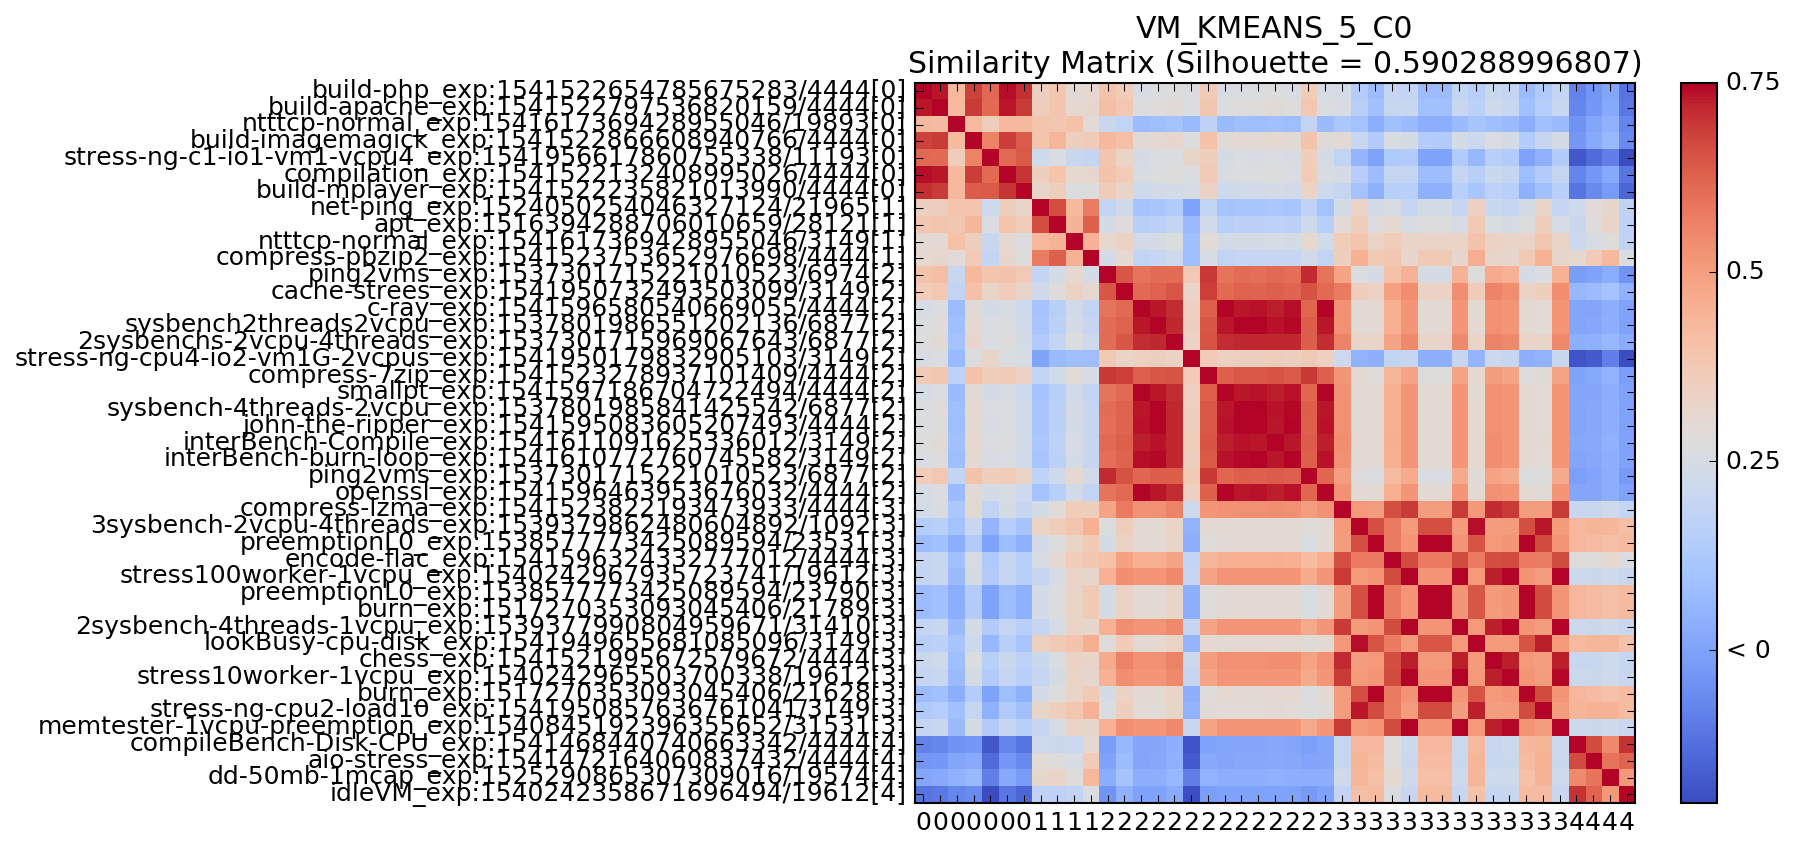
\includegraphics[width=\textwidth]{figs/VM_KMEANS_5_C0.png}
\caption{Similarity Plot For the Five Workload Clusters Discovered in the First Group (Silhouette = 0.59)}
\label{fig:c0-sim}
\end{figure*}
%%%%%%%%%%%%%%%%%%%%%%%%%%%%
%Then use similarity plot to say how good or bad the first group is clustered: note how c2 is packed but c3 or c1 is not and explain. Consider overlapping c2 and c3 and explain why that happens and if it reveals some interesting information (Hani?)

The similarity matrix 

%%%%%%%%%%%%%%%%%%%%%%%%%
\begin{figure*}[!htpb]
\centering
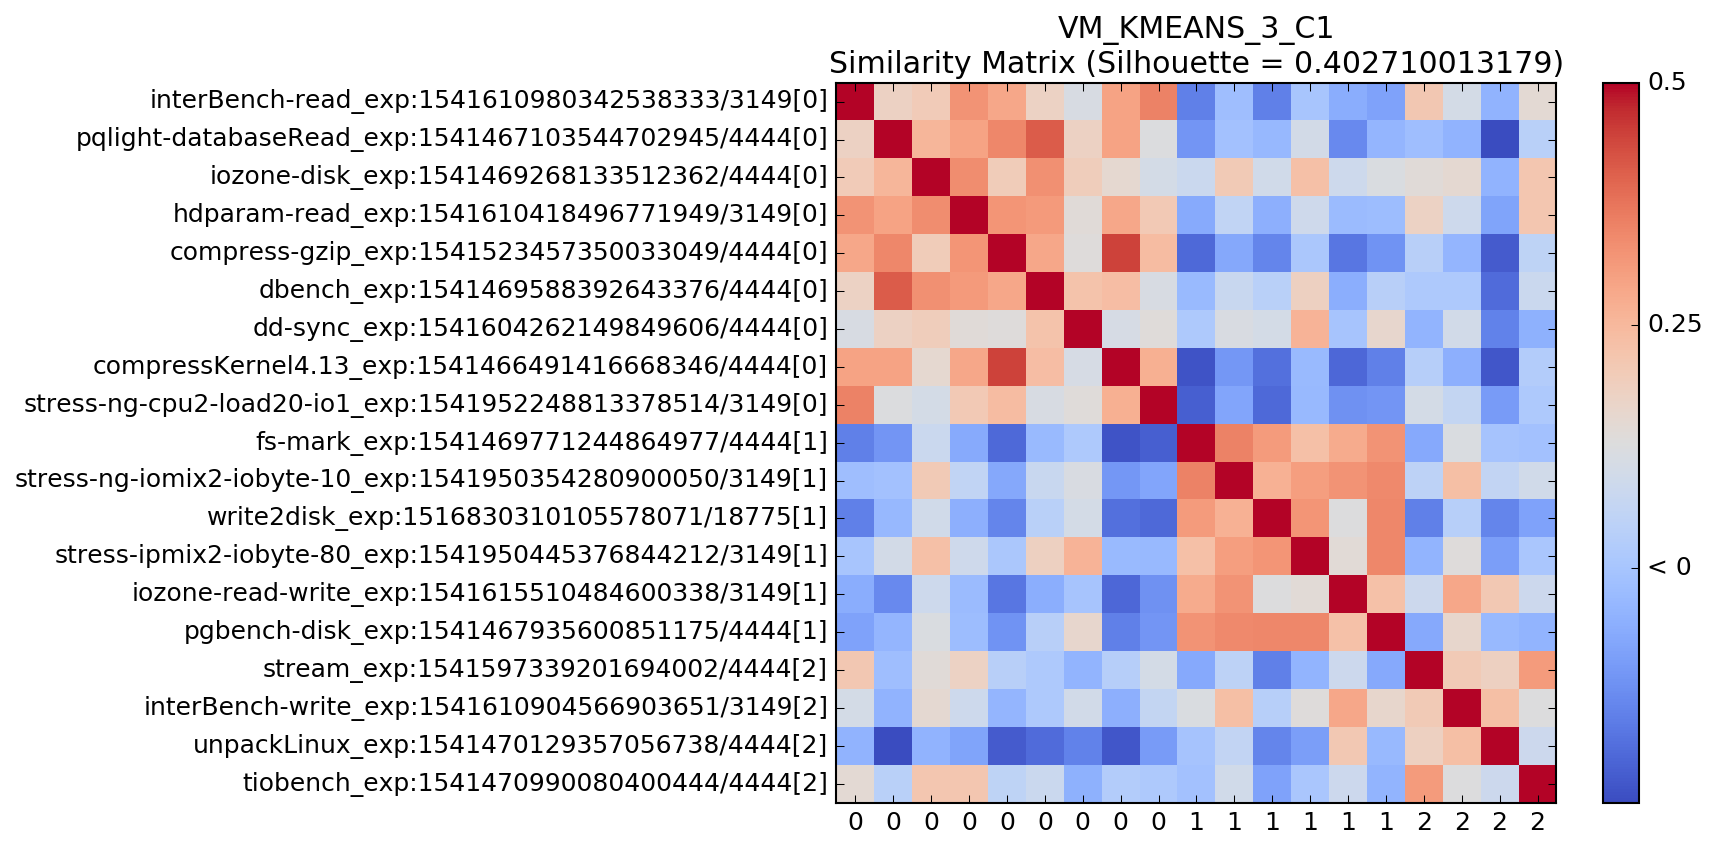
\includegraphics[width=\textwidth]{figs/VM_KMEANS_3_C1.png}
\caption{Similarity Plot For the Three Workload Clusters Discovered in the Second Group (Silhouette = 0.40)}
\label{fig:c1-sim}
\end{figure*}
%%%%%%%%%%%%%%%%%%%%%%%%%%%%
Do the same for second group. More fuzzy group. In particular C2 is very much like noise and uninteresting VM workload. What does this exactly mean for a data center admin? elaborate. 

%%%%%%%%%%%%%%%%%%%%%%%%%
\begin{figure*}[!htpb]
\centering
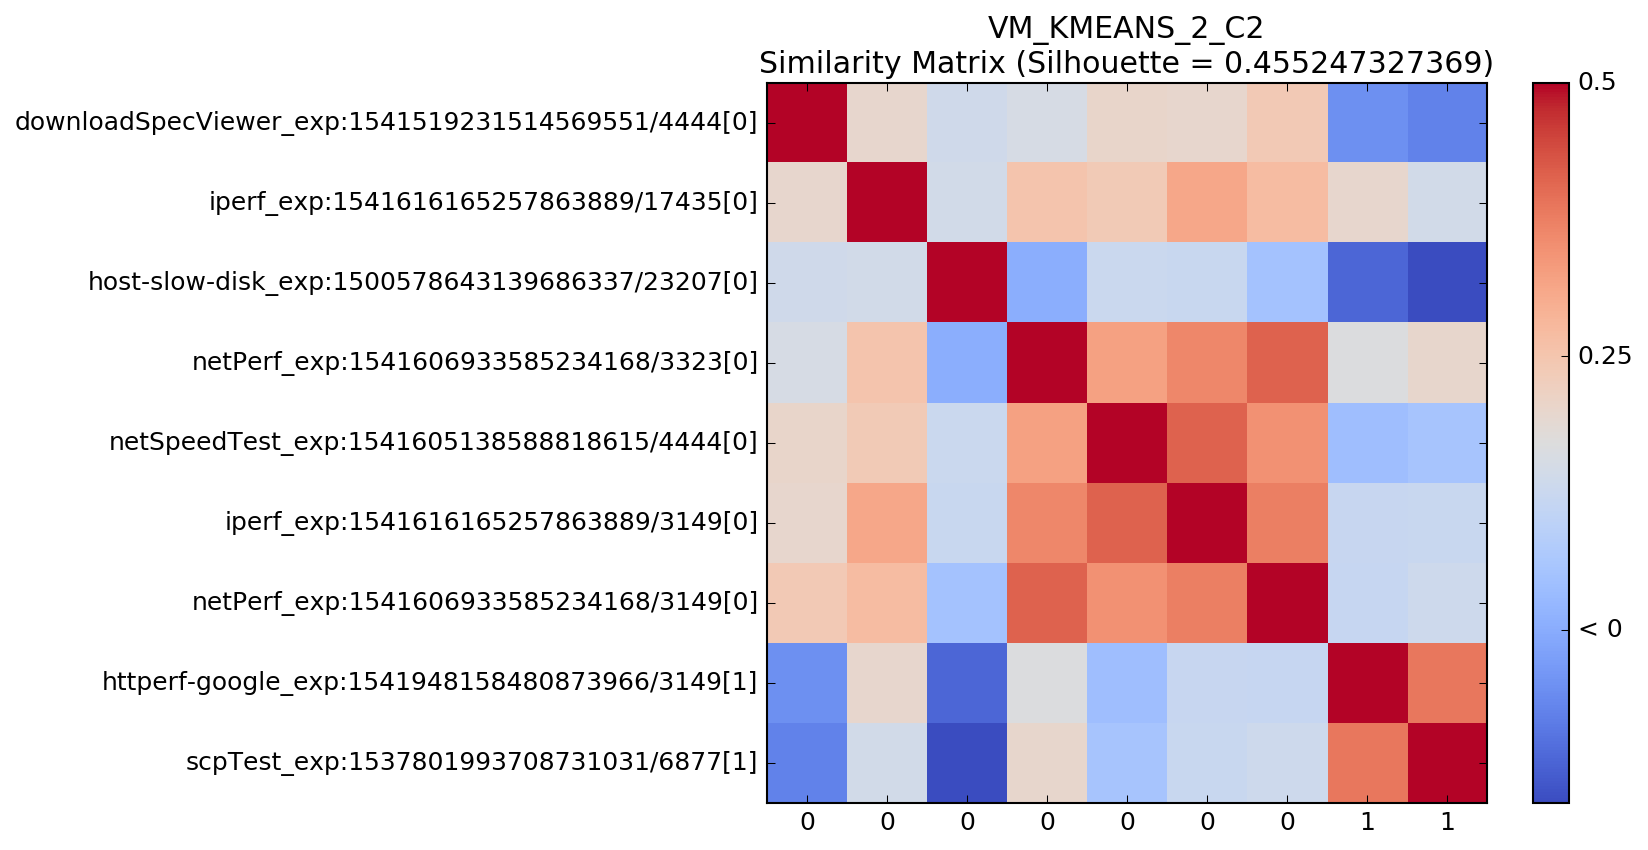
\includegraphics[width=\textwidth]{figs/VM_KMEANS_2_C2.png}
\caption{Similarity Plot For the Two Workload Clusters Discovered in the Third Group (Silhouette = 0.46)}
\label{fig:c2-sim}
\end{figure*}
%%%%%%%%%%%%%%%%%%%%%%%%%%%%
Again the same for third group.

%%%%%%%%%%%%%%%%%%%%%%
\begin{figure*}
	\begin{subfigure}
		\centering
		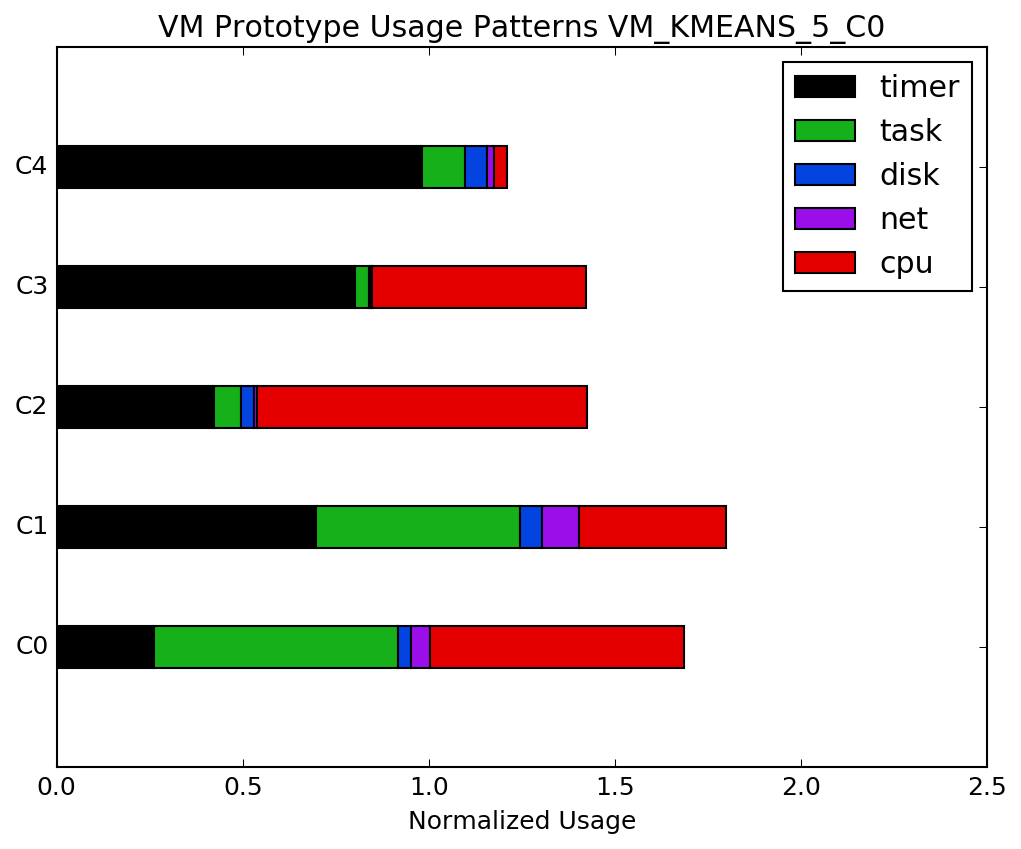
\includegraphics[width=0.3\textwidth]{figs/VM_KMEANS_5_C0_centroids.png}
		\label{fig:c0-centroids}
	\end{subfigure}%
	\begin{subfigure}
		\centering
		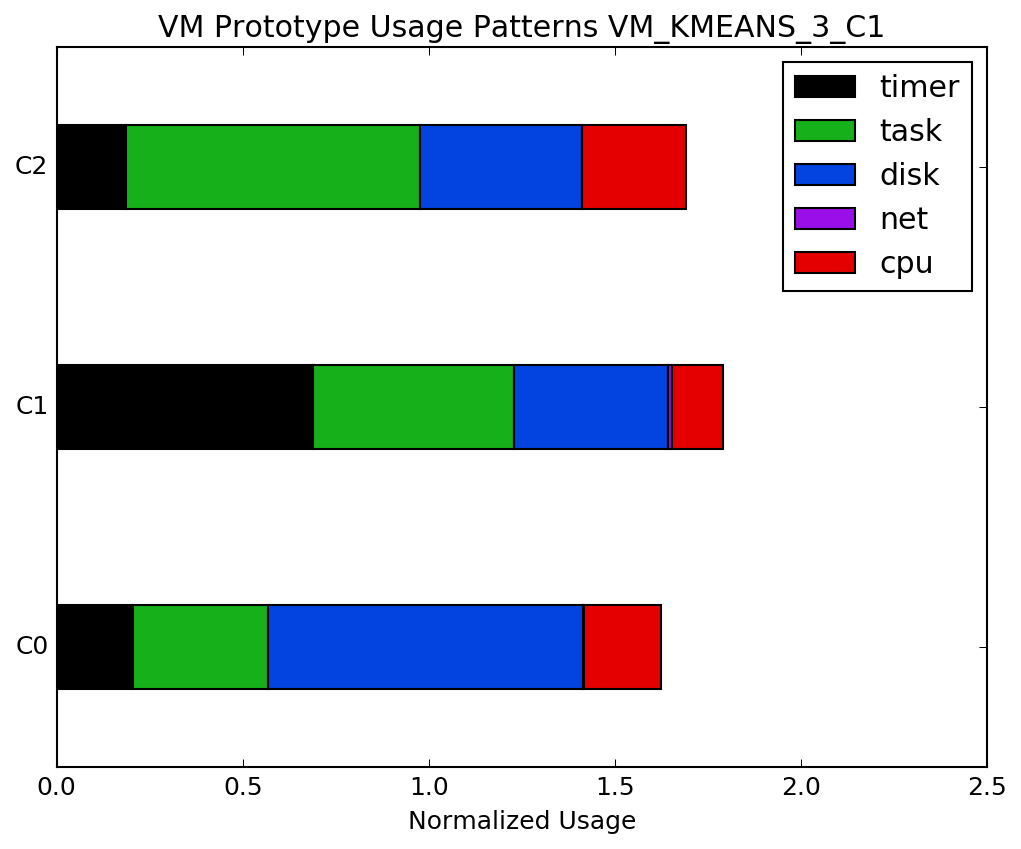
\includegraphics[width=0.3\textwidth]{figs/VM_KMEANS_3_C1_centroids.png}
		\label{fig:c1-centroids}
	\end{subfigure}%
	\begin{subfigure}
		\centering
		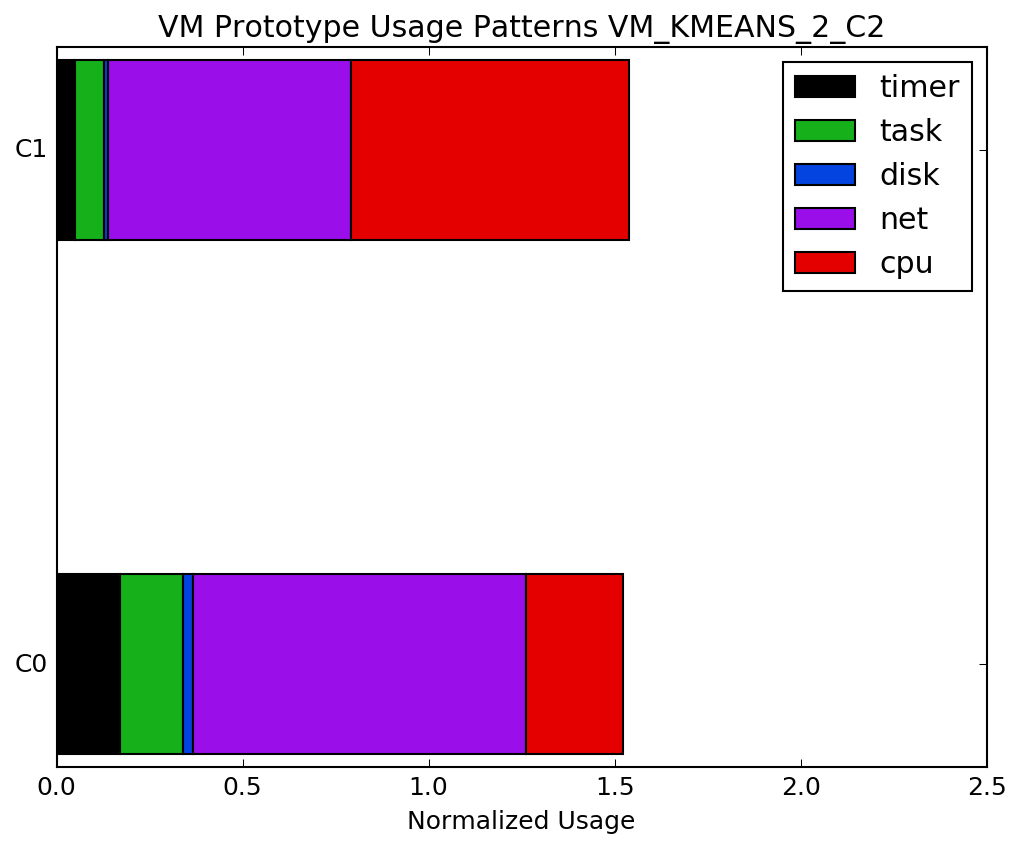
\includegraphics[width=0.3\textwidth]{figs/VM_KMEANS_2_C2_centroids.png}
		\label{fig:c2-centroids}
	\end{subfigure}%
	\caption{Characteristic of Workloads Discovered in Second Stage of Clustering}
	\label{fig:2nd-centroids}
\end{figure*}
%%%%%%%%%%%%%%%%%%%%%%
Now talk about the centroids and how they represent the workload for each cluster.point to interesting and very contrasting cases. How can we take advantage of these diagrams in real life? elaborate (Hani?)

%%%%%%%%%%%%%%%%%%%%%%
\begin{figure*}
	\begin{subfigure}
		\centering
		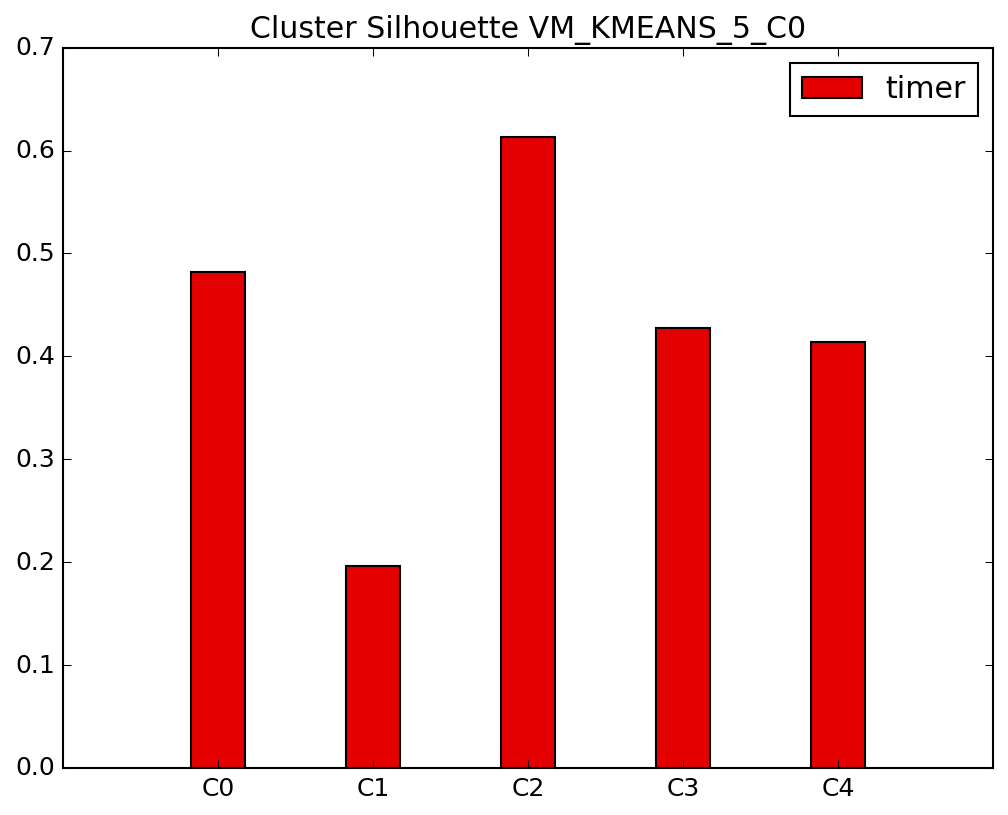
\includegraphics[width=0.3\textwidth]{figs/VM_KMEANS_5_C0_sil.png}
		\label{fig:c0-sil}
	\end{subfigure}%
	\begin{subfigure}
		\centering
		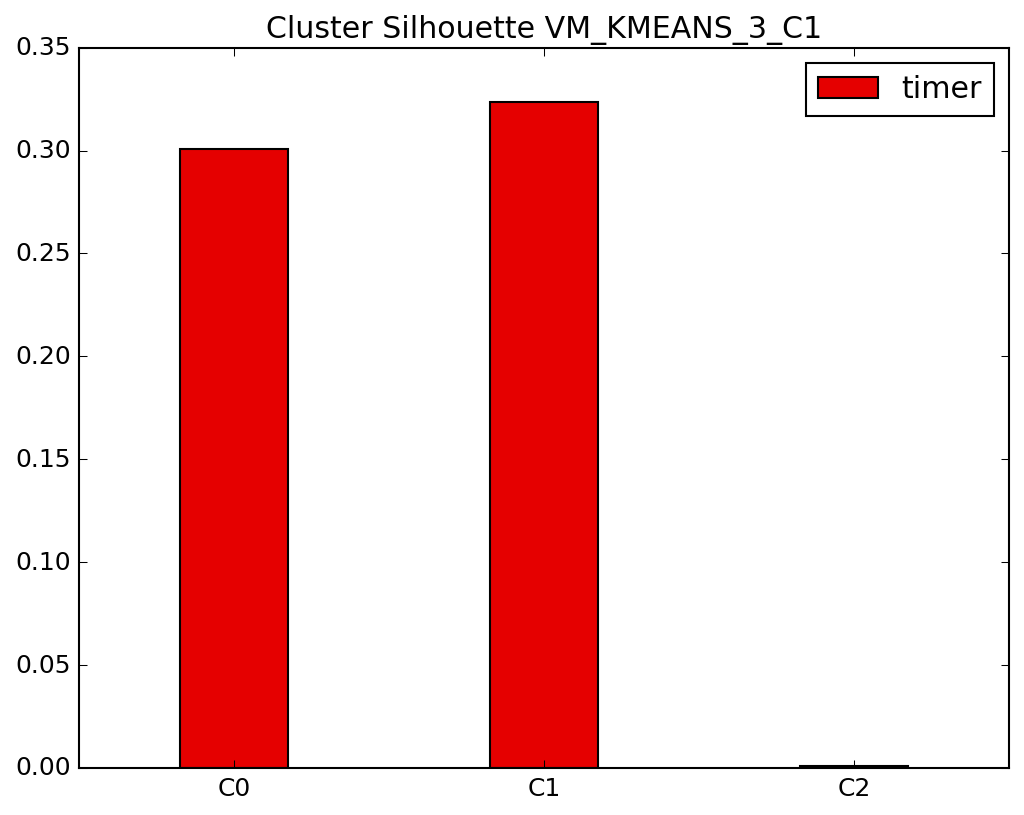
\includegraphics[width=0.3\textwidth]{figs/VM_KMEANS_3_C1_sil.png}
		\label{fig:c1-sil}
	\end{subfigure}%
	\begin{subfigure}
		\centering
		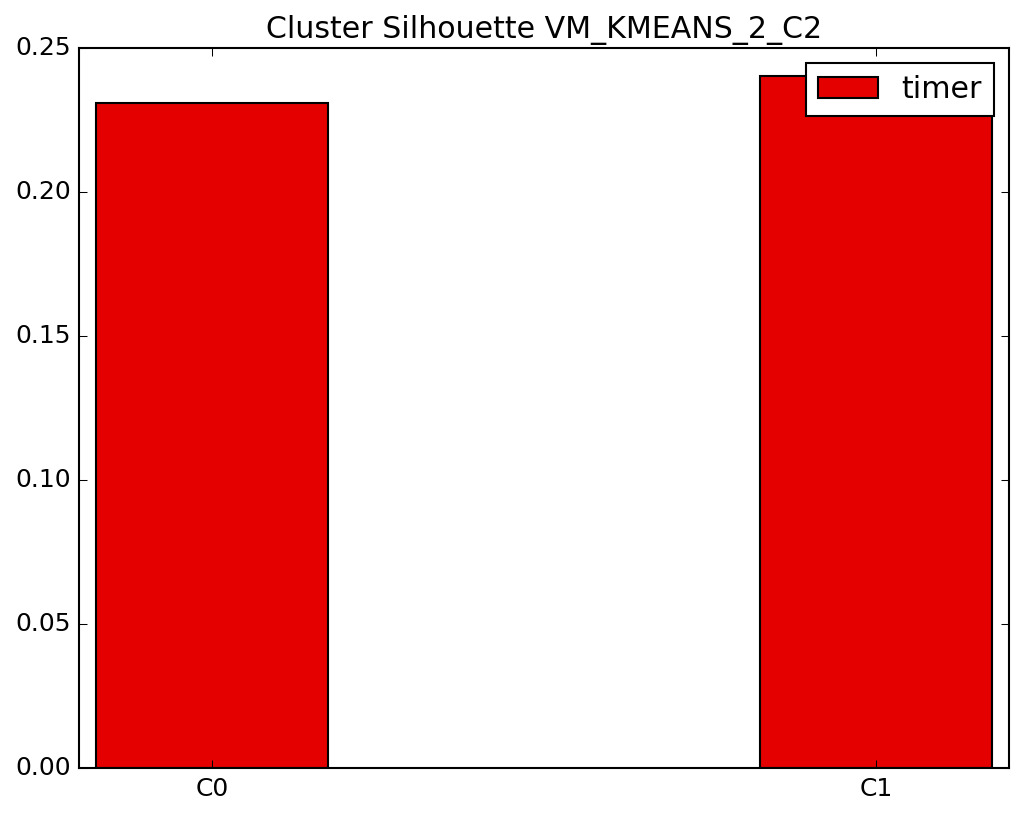
\includegraphics[width=0.3\textwidth]{figs/VM_KMEANS_2_C2_sil.png}
		\label{fig:c2-sil}
	\end{subfigure}%
	\caption{Silhouette Score of VM Clusters Discovered in Second Stage of Clustering}
	\label{fig:2nd-sil}
\end{figure*}
%%%%%%%%%%%%%%%%%%%%%%
These figures \ref{fig:2nd-sil} can assist explaining the similarity matrices. 

%%%%%%%%%%%%%%%%%%%%%%%%%%%%%%%%%%%%%%%%%%%%%%%%%%%%%%%%%%%%%%%%%%%%%%%%%%%%%%%%

\section{Conclusions}






%%%%%%%%%%%%%%%%%%%%%%%%%%%%%%%%%%%%%%%%%%%%%%%%%%%%%%%%%%%%%%%%%%%%%%%%%%%%%%%%
\section*{Acknowledgment}

We would like to gratefully acknowledge the Natural Sciences and Engineering Research Council of Canada (NSERC), Ericsson, Ciena, and EffciOS for funding this project. We thank Genevieve Bastien for her comments.



%%%%%%%%%%%%%%%%%%%%%%%%%%%%%%%%%%%%%%%%%%%%%%%%%%%%%%%%%%%%%%%%%%%%%%%%%%%%%%%%
\bibliographystyle{IEEEtran}
\bibliography{hani}




\end{document}
